\chapter{Evaluation}

\label{ch:evaluation}

\section{Experimental Setup}

The experiments were performed on the department of computing lab machines, $sprite30$ and $sprite29$. These machines have a "HP EliteDesk 800 G2 TWR, Intel Core i7-6700 3.40GHz" CPU and have 16GB of RAM.

\section{Datasets}

\subsection{LDBC Social Network Benchmark Data Generator}

To test our work, we have used the LDBC-SNB DataGen program \cite{Erling:2015:LSN:2723372.2742786}, which generates a social network graph to a number of scale factors. We used scale factors 1, 3 and 10. We would have used larger data but for the size of the machine we performed our experiments with. The number of nodes and edges in these graphs is shown in table \ref{tab:datasets_table}.

\begin{table}[H]
    \centering
    \begin{tabular}{| l | l | l |}
    \hline
    Scale Factor & Nodes & Edges \\ \hline
    1 & 9893 & 180624 \\ \hline
    3 & 24329 & 565248 \\ \hline
    10 & 65646 & 1938517 \\
    \hline
    \end{tabular}
    \caption{LDBC-SNB generated datasets}
    \label{tab:datasets_table}
\end{table}

A major use-case for adaptive indexing on graph data is the prospect of finding trends within a social network. When something happens in the news, for example, the workload changes, requiring a new index to improve performance. We have used a simple popularity/trend-analysis measure in pagerank ("personrank" in our case) to assess the performance of our system.

In this network, people are nodes and their relationships are edges. The node ids are unchanged from the data generation, they are not mapped onto consecutive integers from 0.

\subsection{Randomly Generated Trees}

We wished to find the break-even point of up-front sorting versus our implementations, so to support this, we used breadth-first search on randomly generated trees. To find the "break-even point", we find the time it takes to sort the edge array using quicksort \cite{doi:10.1093/comjnl/5.1.10} and then count the number of queries the cracking implementation has already answered in that time. This is used to determine the gains we can make by using adaptive indexing versus using offline index creation, that is, up-front sorting.

\section{Graph Algorithms}

\subsection{Breadth First Search}

Breadth first search, or BFS, involves choosing a starting node as the sole member of a frontier, which then expands in iterations in which members of the frontier append their out-neighbours which have not yet been visited to the frontier, and remove themselves. This continues until all vertices have been visited.

The most important factor for us in considering BFS is that it queries the outgoing edges of each node just once, meaning that compressed column fragments are never revisited during the course of the algorithm. For this reason we believe it provides an appropriate lower bound on the break-even point.

\subsection{Pagerank}

Pagerank \cite{ilprints422} is a famous algorithm which stores a rank for each vertex and iteratively updates the values across the entire graph. All nodes are initialized with a rank of $\frac{1}{|V|}$. During each iteration, each node inherits from all of its in-neighbours a contribution of their pagerank divided by their out-degree. This value is then multiplied by a damping factor and then added to a base value to give the updated rank. The base value is defined as $\frac{1 - d}{|V|}$.

In pagerank, every iteration considers all of the vertices and edges in the graph, and so over an execution of many iterations, any clustering or compression will see further benefits compared to BFS.

To benchmark our contributions, we have implemented pagerank as an equivalent "personrank" for the generated social network.

\section{Systems under Comparison}

The purpose of this project is not to create the fastest system, but to assess the applicability towards graph processing of compression-based variants of cracking. To ensure that our experiments fairly reflect this, we have chosen to compare our single-threaded cracking implementation to other single-threaded solutions. Predicated and vectorized implementations of cracking have been done and been shown to be highly effective for improving the CPU efficiency of cracking against the original algorithm \cite{Pirk:2014:DCF:2619228.2619232}, however, we have not applied these improvements to our algorithm. This is not a problem because our work is concerned primarily with the fundamental differences between standard cracking and cracking with adaptive compression, rather than optimizing them especially, although we touch on potential optimizations in our discussion of future work.

With that in mind, we have tested our system against the standard cracking algorithm and against upfront quicksort. The reason we have chosen quicksort specifically is for its similarity to cracking, in that it uses pivots to partially sort column sections. Compare this to cracking, which uses pivots to partition the column towards being fully sorted.

Our contributions featured variations in two dimensions: Opportunities to compress and storage of compression information. We have implemented per-fragment compaction, per-fragment recognition, underswapping RLE recognition and overswapping RLE recognition. The reason we decided not to implement compaction with RLE compression is that it seemed clear from the disappointing results of per-fragment compaction that it would not be worth it.

\section{Results}

\subsection{Personrank}

Using data generated by the LDBC-SNB at scale factors of 1, 3 and 10, we measured the wall-clock time to completion of pagerank implementations using each adaptive indexing technique. We have also included the results for an implementation using upfront quicksort.

For each of the three graphs, we ran pagerank over 50 and 100 iterations for every method. Each result is averaged over 10 runs. Blue and red represent the results over 50 and 100 iterations respectively.

\begin{figure}[H]
  \centering
  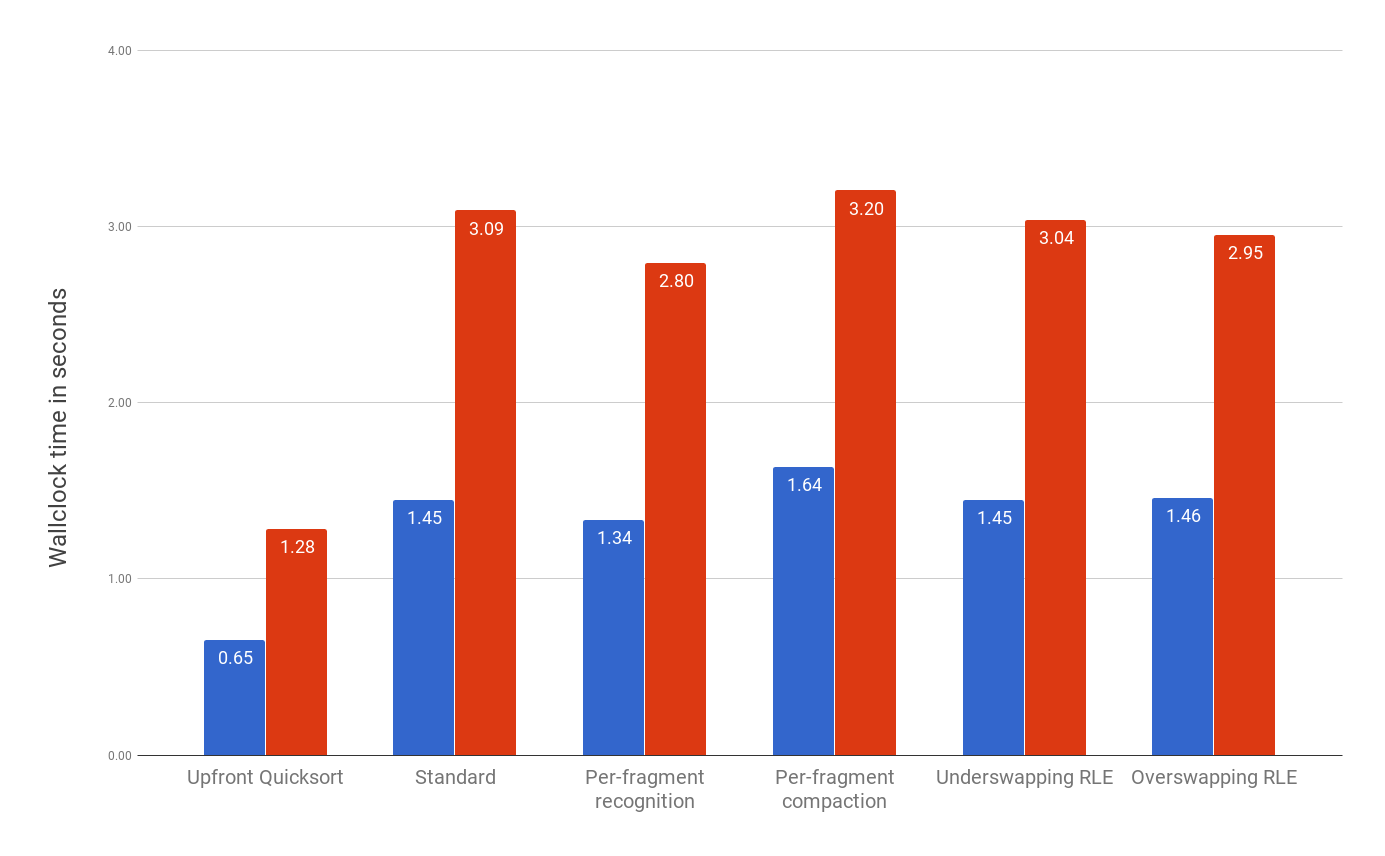
\includegraphics[width=\textwidth]{images/personrankSF1}
  \caption{Personrank execution times for the SF1 social network graph}
  \label{fig:personranksf1}
\end{figure}

\begin{figure}[H]
  \centering
  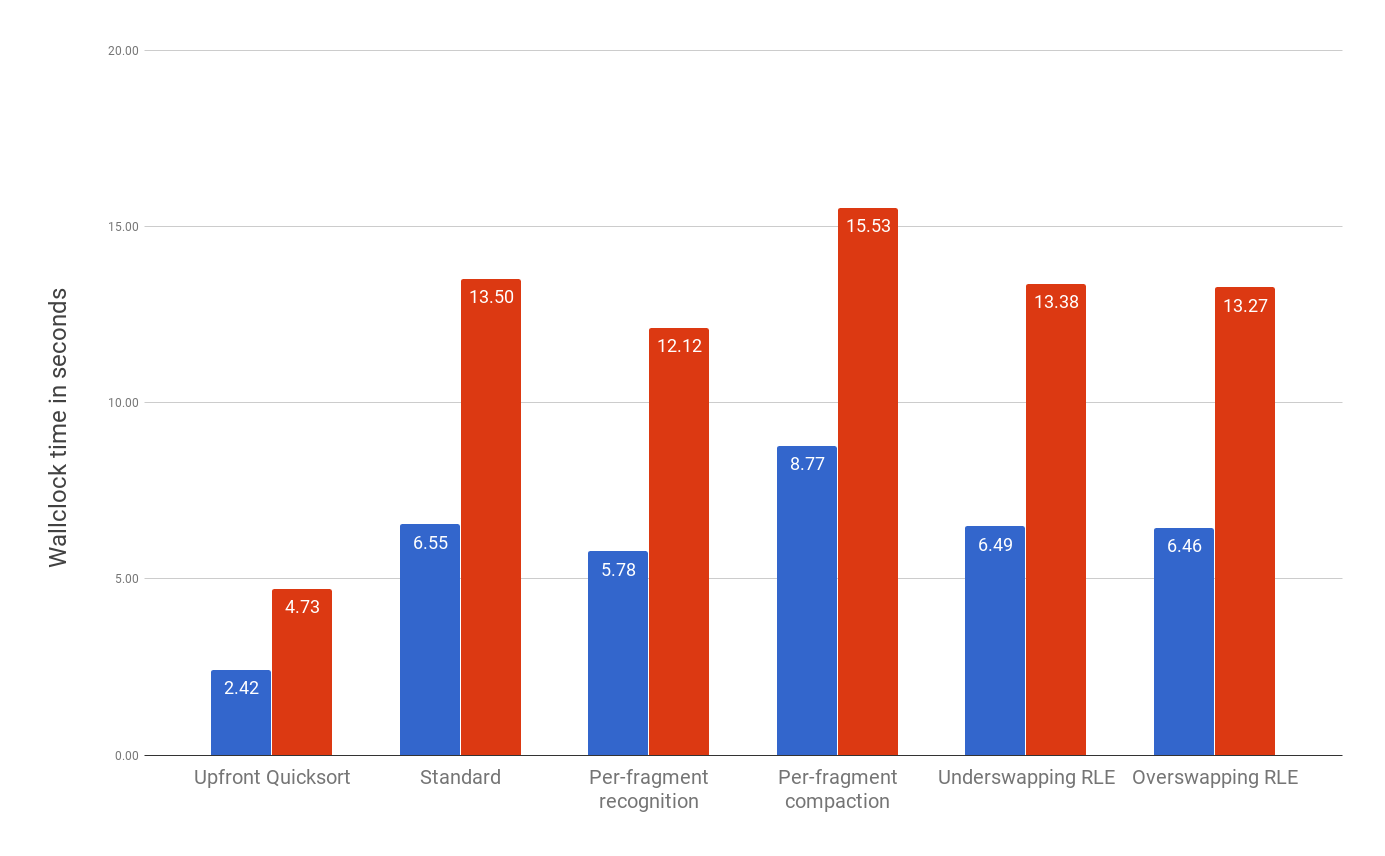
\includegraphics[width=\textwidth]{images/personrankSF3}
  \caption{Personrank execution times for the SF3 social network graph}
  \label{fig:personranksf3}
\end{figure}

\begin{figure}[H]
  \centering
  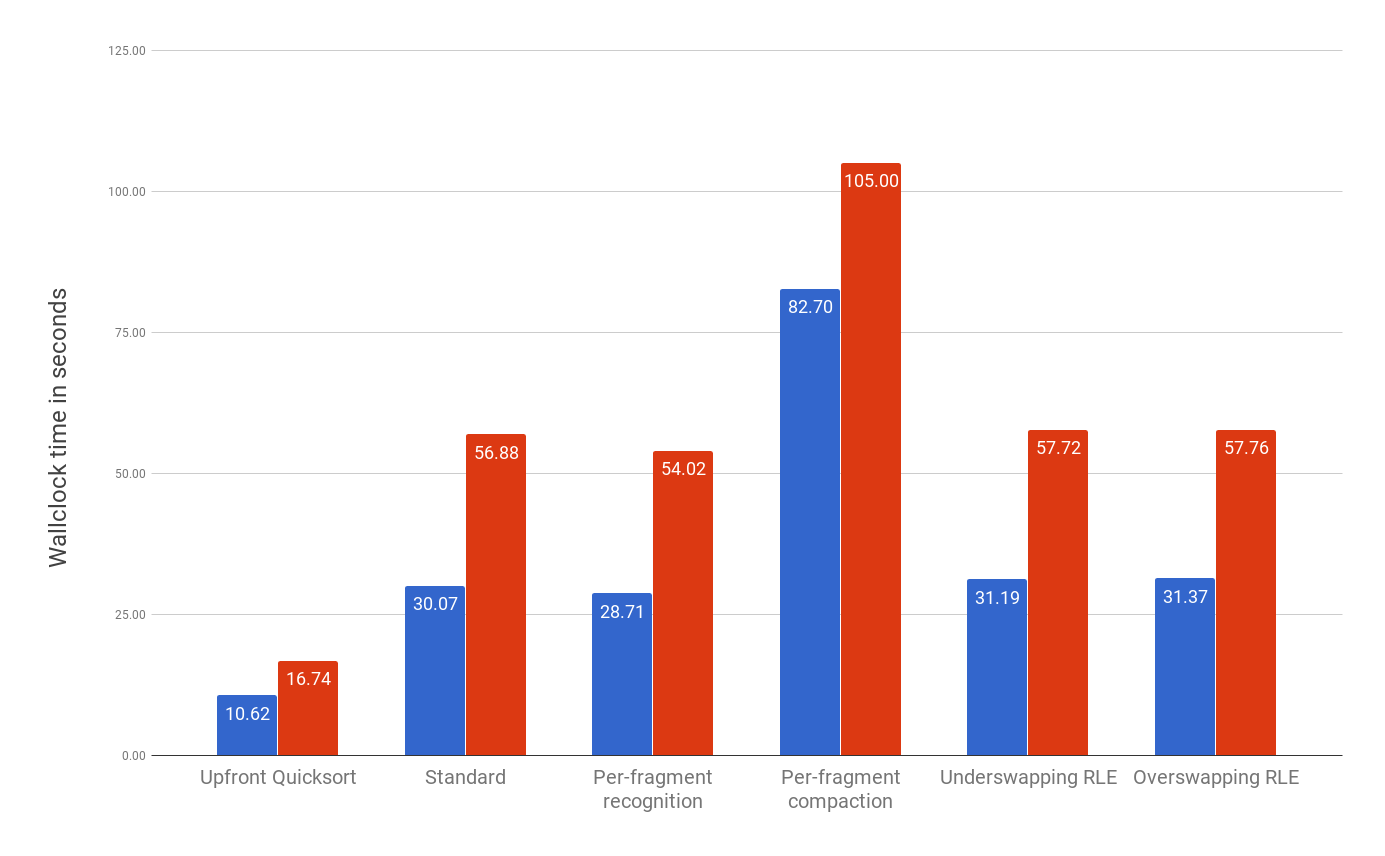
\includegraphics[width=\textwidth]{images/personrankSF10}
  \caption{Personrank execution times for the SF10 social network graph}
  \label{fig:personranksf10}
\end{figure}

Our experiments showed that our implementation of compaction is always the slowest, regardless of data size or the number of iterations. This is due to the prohibitively high costs associated with the constant copying of memory which this technique depends on.

We also showed however, that per-fragment recognition was always the fastest. This is because, by recognizing a uniform column-fragment, we can avoid doing any scanning at all. This optimization to the original algorithm yielded a small average speedup across our six reported executions of 8.1$\%$.

The two RLE methods we developed showed promise. Across our reported executions, they were faster than standard cracking as often as they were slower. We found very little difference in performance between underswapping and overswapping, although this is likely to be because they are inherently very similar, differing only in the way they perform high-side swaps of two runs of different lengths - a case which is evidently not encountered enough to show any sizable performance difference between the two different implementations of that case.

\subsection{Break-even Point}

Using randomly generated trees, we ran BFS using each adaptive method and counted how many cracking queries were completed in the same amount of time as it took to sort the tree using quicksort.

The reason we chose to do BFS on trees, is that it represents a case in which every query is guaranteed to be doing a scan and not returning compressed values. We did this in order to assess how much of an impact on the break-even performance and early-scanning speed our changes had to the original cracking algorithm.

We evaluated the break-even point for trees of size 100,000, 500,000 and 1,000,000 (number of nodes), averaged over 10 runs, with a new tree for each run. Our results are shown in figure \ref{fig:breakeven}. Blue, red and yellow represent the results for the trees with 100,000, 500,000 and 1,000,000 nodes respectively.

\begin{figure}[h]
  \centering
  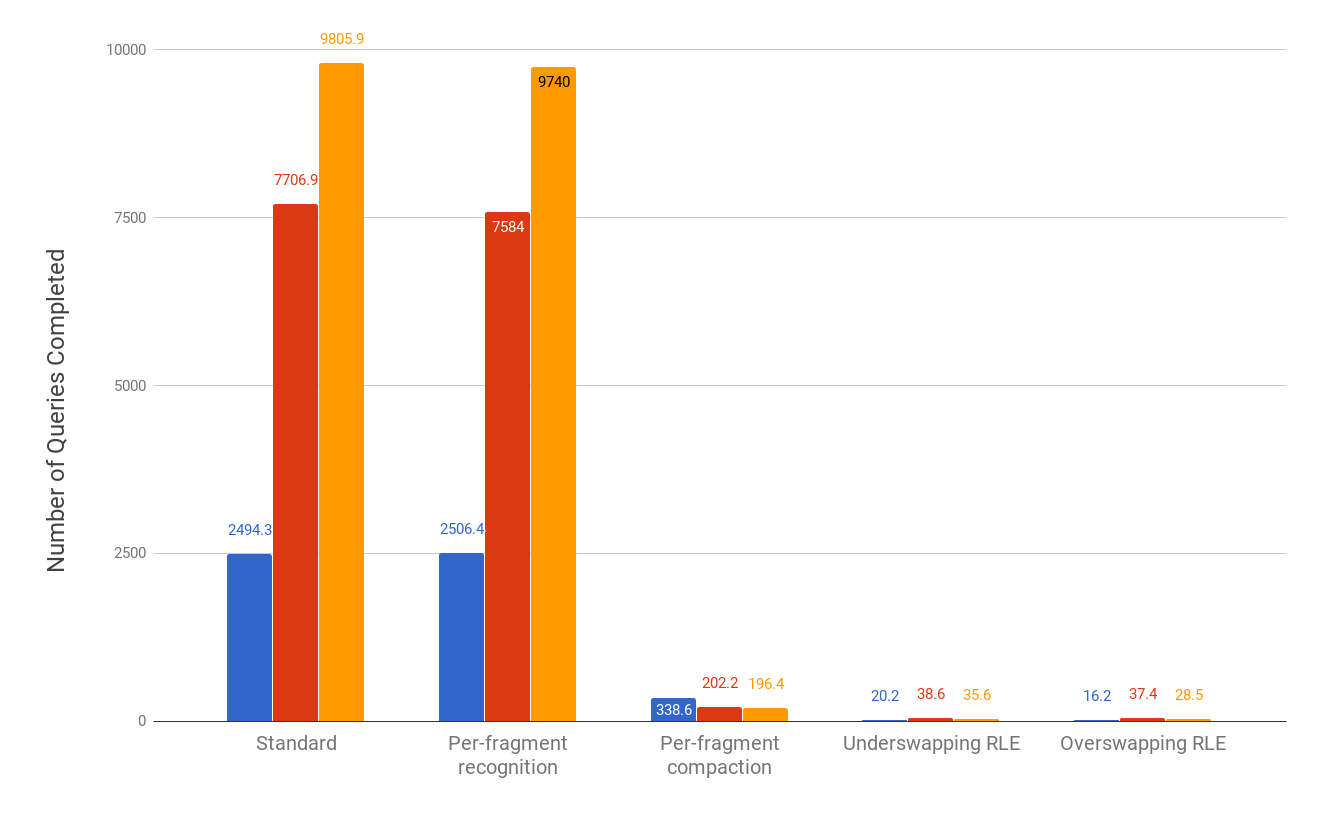
\includegraphics[width=\textwidth]{images/breakeven}
  \caption{Break-even point for each studied adaptive technique}
  \label{fig:breakeven}
\end{figure}

Compaction performed poorly compared to standard cracking in this test. We see that with greater data size, the number of queries ran by compaction in the same time as it took to sort the array decreases. This makes sense given that the primary cost factor in compaction is the copying of memory. As the size of the array increases and the number of copied values increases, so the performance during early queries will decrease.

Per-fragment recognition makes no changes to the cracking scan, and so it makes sense that there would be little difference in the break-even point compared to standard cracking, regardless of the data size.

The two RLE cracking variants actually change the implementation of the scan - they perform extra work to build and maintain knowledge about runs in exchange for the ability to exploit this knowledge. In the early queries we expect the costs to outweigh the benefits, because at the start, there is no run-length information to exploit, but at the same time there is a lot of new information to build and write into memory, which is expensive. This results in a significantly higher relative cost for early queries when using RLE cracking, causing the break-even point to be dramatically lower. This is unfortunate, because one of the main advantages of using cracking over a non-adaptive indexing technique is that it is lightweight - a property lost by performing expensive run-length encoding in early queries.

Compared to overswapping, underswapping performs less work during high-side swapping. It has fewer branches because it does not have to deal with padding or overlapping. The earliest queries perform the largest scans and therefore perform the most swaps. It therefore makes sense that the relative advantage underswapping has in performing less work during swapping would be most evident in the earliest queries.

\subsection{Summary}

\begin{itemize}
\item \textbf{Per-fragment Compaction}: This method was quite disappointing, although it cannot be said that it was unexpected. The costs of deleting arbitrary elements from an array and copying the non-contiguous data towards the head are too high to make this a viable technique.
\item \textbf{Per-fragment Recognition}: By recognizing uniform column pieces using the invariants of the cracker index, we can prevent unnecessary scans, which improves performance. We showed that per-fragment recognition is an effective way to improve the performance of cracking as an adaptive index on an edge-array representing a graph.
\item \textbf{RLE}: We showed that run-length encoding an edge array during cracking is a technique that performs similarly to standard cracking in terms of overall speed, but is a far less lightweight operation.
\end{itemize}